\chapter{A-A WEAPONS}
\thumbtab{A-A}{5}
\minitoc
\cleardoublepage

\section{M-61 CANNON}

\subsection{OVERVIEW}
\mbox{
    \begin{minipage}[t][25mm][c]{\textwidth}
        \centering
        \LARGE\emph{IMAGE PLACEHOLDER}
    \end{minipage}
}
\begin{tableitemize}
    \blueitem{M-61}{
    \begin{subitemize}
        \item \textbf{Fire Rate} -- 6000rpm
        \item \textbf{Round Size} -- 20mm
        \item \textbf{Ammo Capacity} -- 510 rounds
    \end{subitemize}}
    \blueitem{Ammunition Types}{
    \begin{subitemize}
        \item \textbf{HEI} -- \textbf{H}igh \textbf{E}xplosive \textbf{I}ncendiary
        \item \textbf{HEI-T} -- \textbf{H}igh \textbf{E}xplosive \textbf{I}ncendiary-\textbf{T}racer
        \item \textbf{AP} -- \textbf{A}rmor \textbf{P}iercing
        \item \textbf{TP} -- \textbf{T}arget \textbf{P}ractice
        \item \textbf{SAPHEI} -- \textbf{S}emi \textbf{A}rmor \textbf{P}iercing \textbf{H}igh \textbf{E}xplosive \textbf{I}ncendiary
    \end{subitemize}}
    \blueitem{Select GUN}{
    \emph{Via MFD}

    \begin{subenumerate}
        \item \textbf{Master Mode} \dotfill \textbf{A-A}
        \item \textbf{Selected Weapon} \dotfill \textbf{GUN}
        \begin{itemize}
            \item \textbf{Cycle} -- Press \textbf{OSB 7}
        \end{itemize}
    \end{subenumerate}
    
    \emph{Via Dogfight}

    \begin{subenumerate}
        \item \textbf{DGFT/MSL OVRD} \dotfill \textbf{DGFT}
        \begin{itemize}
            \item AIM-9 \& GUN automatically selected
        \end{itemize}
    \end{subenumerate}}
\end{tableitemize}

\subsection{SYMBOLOGY}

\clearpage

\subsection{GUN EMPLOYMENT}
\begin{tablenumerate}
    \blueitem{Conditions}{
    \begin{subitemize}
        \item \textbf{FCR} \dotfill \textbf{ON}
        \item \textbf{RF Switch} \dotfill \textbf{NORM} \\
        \hfill (If radar use desired)
        \item \textbf{Selected Weapon} \dotfill \textbf{GUN} \\
        \hfill (or \textbf{DGFT} selected)
        \item \textbf{Master Arm} \dotfill \textbf{ARM}
    \end{subitemize}}
    \blueitem{Radar \break Acquisition}{
    \begin{subitemize}
        \item Acquire lock using desired \textbf{ACM Mode}
        \item Also possible from \textbf{CRM-STT} mode
    \end{subitemize}}
    \blueitem{Symbology}{
    \begin{subitemize}
        \item \textbf{EEGS LVL II} -- appears upon gun selection
        \item \textbf{EEGS LVL V} -- appears on radar lock
    \end{subitemize}}
    \blueitem{Employment}{
    \emph{With Radar}

    \begin{subenumerate}
        \item \textbf{Radar} \dotfill Locked
        \item \textbf{Maneuver} -- Place pipper over target
        \item \textbf{Fire Gun} \dotfill \textbf{TRIGGER 2nd Detent}
    \end{subenumerate}
    
    \emph{Without Radar}

    \begin{subenumerate}
        \item \textbf{Maneuver} -- Place target within funnel
        \begin{itemize}
            \item \textbf{Range} -- Tgt wingtips on funnel lines
        \end{itemize}
        \item \textbf{Fire Gun} \dotfill \textbf{TRIGGER 2nd Detent}
    \end{subenumerate}}
    \blueitem{Drafting Notes}{
    \begin{subitemize}
        \item Figure showing generic EEGS II with labels in the overview and one showing ``mid-pull'' with target in range here would be great
        \item Figure showing EEGS V ``mid-pull'' with target under pipper for this page
        \item Would be great to have separate diagrams for TMS functions for each sensor/mode, then can paste that here as well as reminder
    \end{subitemize}}
\end{tablenumerate}

\clearpage

\section{AIM-9 SIDEWINDER}

\subsection{OVERVIEW}
\mbox{
    \begin{minipage}[t][25mm][c]{\textwidth}
        \centering
        \LARGE\emph{IMAGE PLACEHOLDER}
    \end{minipage}
}
\begin{tableitemize}
    \blueitem{AIM-9}{
    \begin{subitemize}
        \item \textbf{Guidance} -- IR-guided (\textbf{Fox 2})
        \item \textbf{Range} -- min: \textasciitilde3000ft, max: \textasciitilde10-20nm
    \end{subitemize}}
    \blueitem{Variants}{
    \begin{subitemize}
        \item \textbf{9M} -- IR-guided, short range, all-aspect
        \item \textbf{9X} -- HOBS (\textbf{H}igh \textbf{O}ff-\textbf{B}ore\textbf{S}ight) capable
    \end{subitemize}}
    \blueitem{Acquisition / Cueing Modes}{
    \begin{subitemize}
        \item Seeker slaved to radar track LOS \\
        \hyperref[subsec:aim9slave]{\textbf{See \Cref{subsec:aim9slave}}}
        \item Acquisition with own missile seeker \\
        \hyperref[subsec:aim9bore]{\textbf{See \Cref{subsec:aim9bore}}}
        \item Seeker cued with HMD LOS \\
        \textbf{Possible in either \hyperref[subsec:aim9slave]{\textbf{Slaved}} or \hyperref[subsec:aim9bore]{\textbf{Bore}} mode}
    \end{subitemize}}
    \blueitem{SMS Page}{\textbf{See Figure X.XX} and below items}
    \blueitem{SPOT / SCAN}{
    \begin{subitemize}
        \item \textbf{Controls Seeker Field of View}
        \item \textbf{SPOT} -- Narrow, increased detection range
        \item \textbf{SCAN} -- Wide, decreased detection range
    \end{subitemize}}
    \blueitem{SLAVE / BORE}{
    \begin{subitemize}
        \item \textbf{Controls Seeker Line of Sight}
        \item \textbf{SLAVE} - \hyperref[subsec:aim9slave]{\textbf{See \Cref{subsec:aim9slave}}}
        \begin{itemize}
            \item Seeker slaved to radar track LOS \\
            \item Typically via ACM Modes \\
            (including HMD, if powered)
        \end{itemize}
        \item \textbf{BORE} - \hyperref[subsec:aim9bore]{\textbf{See \Cref{subsec:aim9bore}}}
        \begin{itemize}
            \item Acquisition with own missile seeker
            \item Or cued with HMD (if powered)
            \item \textbf{Does NOT require FCR}
        \end{itemize}
    \end{subitemize}}
    \blueitem{WARM / COOL}{
    \begin{subitemize}
        \item \textbf{Controls Seeker Cooling Status}
        \item \textbf{COOL} --  increases seeker sensitivity, should be set prior to engagement
        \item Set automatically for \textbf{DGFT} \& \textbf{MSL OVRD}
    \end{subitemize}}
    \blueitem{Select AIM-9}{
    \emph{Via MFD}

    \begin{subenumerate}
        \item \textbf{Master Mode} \dotfill \textbf{A-A}
        \item \textbf{Selected Weapon} \dotfill \textbf{9LM / 9X}
        \begin{itemize}
            \item \textbf{Cycle} -- \textbf{OSB 7} or long press \textbf{NWS}
        \end{itemize}
    \end{subenumerate}
    
    \emph{Via Dogfight}

    \begin{subenumerate}
        \item \textbf{DGFT/MSL OVRD} \dotfill \textbf{DGFT}
        \begin{itemize}
            \item AIM-9 \& GUN automatically selected
        \end{itemize}
        \item \textbf{Selected Weapon} \dotfill Verify \textbf{9LM / 9X}
    \end{subenumerate}}
    \blueitem{Selected Station}{}
\end{tableitemize}

\notebox{
    \begin{itemize}
        \item \textbf{Behavior with SLAVE selected but no radar lock}
        \item \textbf{Is HMD BORE cueing only possible with 9X?}
    \end{itemize}
}

\clearpage

\subsection{SYMBOLOGY}
\begin{tableitemize}
    \blueitem{HUD Symbology}{}
\end{tableitemize}

\clearpage

\subsection{9M/9X - SLAVE - RADAR}
\label{subsec:aim9slave}
\begin{tablenumerate}
    \blueitem{Conditions}{
    \begin{subitemize}
        \item \textbf{FCR} \dotfill \textbf{ON}
        \item \textbf{RF Switch} \dotfill \textbf{NORM}
        \item \textbf{HMD SYMB. INT} \dotfill As desired
        \item \textbf{Selected Weapon} \dotfill \textbf{9M/9X}
        \item \textbf{SLAVE/BORE} \dotfill Verify \textbf{SLAVE}
        \item \textbf{Master Arm} \dotfill \textbf{ARM}
    \end{subitemize}}
    \blueitem{Radar \break Acquisition}{
    \begin{subitemize}
        \item Acquire lock using desired \textbf{ACM Mode}
        \item Also possible from \textbf{CRM-STT} mode
    \end{subitemize}}
    \blueitem{Symbology}{
    \begin{subitemize}
        \item 
    \end{subitemize}}
    \blueitem{Employment}{
    \begin{subenumerate}
        \item \textbf{Radar} \dotfill Locked
        \item \textbf{CAGE/UNCAGE} \dotfill \textbf{Depress}
        \begin{itemize}
            \item \textbf{MSL Diamond} -- Latched to target
            \item \textbf{Audio Tone} -- Verify Good
        \end{itemize}
        \item \textbf{Maneuver} -- Place target within DLZ
        \item \textbf{WPN REL} \dotfill \textbf{Depress}
    \end{subenumerate}}
\end{tablenumerate}

\clearpage

\subsection{9M/9X - BORE - NO RADAR}
\label{subsec:aim9bore}
\begin{tablenumerate}
    \blueitem{Conditions}{
    \begin{subitemize}
        \item \textbf{HMD SYMB. INT} \dotfill As desired
        \item \textbf{Selected Weapon} \dotfill \textbf{9M/9X}
        \item \textbf{SLAVE/BORE} \dotfill \textbf{BORE}
        \item \textbf{Master Arm} \dotfill \textbf{ARM}
    \end{subitemize}}
    \blueitem{Symbology}{
    \begin{subitemize}
        \item 
    \end{subitemize}}
    \blueitem{Employment}{
    \begin{subenumerate}
        \item \textbf{Maneuver} -- Target in AC/HMD boresight
        \begin{itemize}
            \item \textbf{Audio Tone} -- Verify Good
        \end{itemize}
        \item \textbf{CAGE/UNCAGE} \dotfill \textbf{Depress}
        \begin{itemize}
            \item \textbf{MSL Diamond} -- Latched to target
            \item \textbf{Audio Tone} -- Verify Good
        \end{itemize}
        \item \textbf{Maneuver} -- Place target within DLZ
        \item \textbf{WPN REL} \dotfill \textbf{Depress}
    \end{subenumerate}}
\end{tablenumerate}

\clearpage 

\section{AIM-120 AMRAAM}

\begin{figure}[h]
    \centering
    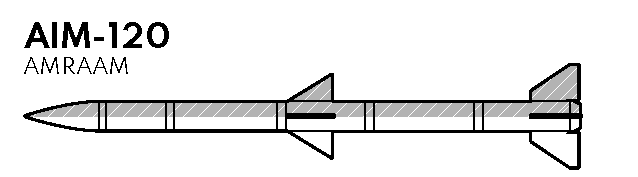
\includegraphics[
            width = 108mm,
    ]{F16_aaweapons_amraam_overview_v01.pdf}
    \caption{}
\end{figure}

\begin{figure}[h]
    \centering
    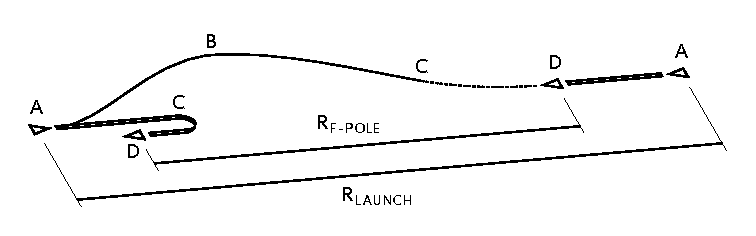
\includegraphics[
            width = 128mm,
    ]{F16_aaweapons_amraam_employment_v07.pdf}
    \caption{}
\end{figure}

\subsection{OVERVIEW}

\begin{tableitemize}
    \blueitem{AIM-120}{
    \begin{subitemize}
        \item \textbf{Guidance} -- Active Radar-Guided (\textbf{Fox 3})
        \item \textbf{Range} -- max:  \textasciitilde30-40nm (high mach, alt)
    \end{subitemize}}
    \blueitem{Engagement \break Types}{
    \begin{subitemize}
        \item \textbf{Single Target} -- \hyperref[subsec:aim120single]{\textbf{See \Cref{subsec:aim120single}}}
        \begin{itemize}
            \item From STT radar lock
        \end{itemize}
        \item \textbf{Multi Target} -- \hyperref[subsec:aim120multi]{\textbf{See \Cref{subsec:aim120multi}}}
        \begin{itemize}
            \item For TWS tracks
            \item Or DTT tracks
        \end{itemize}
    \end{subitemize}}
    \blueitem{SMS Page}{\textbf{See Figure X.XX} and below items}
    \blueitem{SLAVE / BORE}{
    \begin{subitemize}
        \item \textbf{Controls Missile Radar Line of Sight}
        \item \textbf{SLAVE}
        \begin{itemize}
            \item Missile LOS slaved to AC radar 
            \item Receives DL updates until within own radar limits
        \end{itemize}
        \item \textbf{BORE}
        \begin{itemize}
            \item Missile scans straight ahead, tracks first detected target
        \end{itemize}
    \end{subitemize}}
    \blueitem{Select AIM-120}{
    \emph{Via MFD}

    \begin{subenumerate}
        \item \textbf{Selected Weapon} \dotfill \textbf{120C}
        \begin{itemize}
            \item \textbf{Cycle} -- \textbf{OSB 7} or long press \textbf{NWS}
        \end{itemize}
    \end{subenumerate}

    \emph{Via Missile Override}

    \begin{subenumerate}
        \item \textbf{DGFT/MSL OVRD} \dotfill \textbf{MSL OVRD}
        \item \textbf{Selected Weapon} \dotfill Verify \textbf{120C} 
    \end{subenumerate}
    
    \emph{Via Dogfight}

    \begin{subenumerate}
        \item \textbf{DGFT/MSL OVRD} \dotfill \textbf{DGFT}
        \item \textbf{Selected Weapon} \dotfill \textbf{120C}
        \begin{itemize}
            \item \textbf{Cycle} -- \textbf{OSB 7} or long press \textbf{NWS}
        \end{itemize}
    \end{subenumerate}}
    \blueitem{Selected Station}{}
\clearpage

\subsection{EMPLOYMENT PROFILE}

\begin{figure}[h]
    \centering
    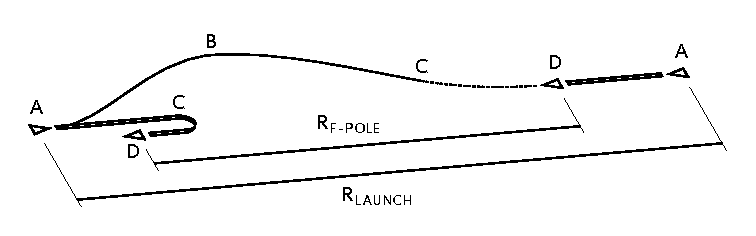
\includegraphics[
            width = 128mm,
    ]{F16_aaweapons_amraam_employment_v07.pdf}
    \caption{Generic, simplified AIM-120 employment profile}
    \label{fig:aa-weap:aim120:profile}
\end{figure}

\begin{tcoloritemize}
    \blueitem{Phases}{
    \Cref{fig:aa-weap:aim120:profile} shows AIM-120 employment profile
    including the following phases \& milestones

    \begin{subitemize}
        \item \textbf{A} -- Launch
        \item \textbf{B} -- Mid-Course Phase
        \item \textbf{C} -- Acquisition
        \item \textbf{D} -- Intercept
    \end{subitemize}}
    \blueitem{Launch}{
    Radar Lock

    \begin{subitemize}
        \item Only requires track to launch
        \item Target does \textbf{NOT} need to be in STT lock
    \end{subitemize}

    Maximizing Range -- maximizing energy

    \begin{subitemize}
        \item High velocity -- increases kinetic energy
        \item High altitude -- increases potential energy, reduces drag
    \end{subitemize}

    Lofting 

    \begin{subitemize}
        \item At longer ranges the missile will loft itself to optimize trajectory
        \item Pilot can manually loft by raising the nose 20-30 deg prior to launch
    \end{subitemize}}
    \blueitem{Mid-Course Phase}{
    Missile flies using internal IMU

    \begin{subitemize}
        \item Receives periodic datalink updates
        \item Will fly to last updated target position if DL lost
    \end{subitemize}}
    \blueitem{Acquisition \& MPRF ``Active'' Phase}{
    Once close to DL bandit location
    \begin{subitemize}
        \item AIM-120 radar turns on in MPRF (Medium Pulse Repetition Frequency) mode 
        \item Locks on to closest / best target
    \end{subitemize}}
    \blueitem{Terminal Phase \& Intercept}{
    Once missile has gone active
    \begin{subitemize}
        \item Flies a PNG intercept trajectory to intercept the target locked by it's radar 
        \item Requires no support from launching fighter which can now turn commpletely away from the bandit
    \end{subitemize}}
\end{tcoloritemize}

\notebox{
    \textbf{Cranking}
    \begin{itemize}
            \item For simplicity, \cref{fig:aa-weap:aim120:profile} does not show any post-launch maneuvers until point \textbf{C}, where the missile goes active 
            \item Depending on the tactical situation, it can be beneficial to reduce closure by turning 30-60 deg away from the bandit while maintaing radar contact 
            \item This can be combined with a dive into thicker air to further reduce bandit missile range and maintain a look-up angle for the radar
    \end{itemize}
    \textbf{Flowing Cold}
    \begin{itemize}
        \item The fighter can turn cold prior to the missile going active
        \item Missile will fly to last DL target position, significantly reducing probability of intercept
    \end{itemize}
}

\clearpage

\subsection{SYMBOLOGY}
\begin{tableitemize}
    \blueitem{HUD Symbology}{}
    \blueitem{FCR Symbology}{}
\end{tableitemize}

\clearpage

\subsection{SINGLE TARGET EMPLOYMENT}
\label{subsec:aim120single}
\begin{tablenumerate}
    \blueitem{Conditions}{
    \begin{subitemize}
        \item \textbf{FCR} \dotfill \textbf{ON}
        \item \textbf{RF Switch} \dotfill \textbf{NORM}
        % \item \textbf{Master Mode} \dotfill \textbf{A-A}
        \item \textbf{Selected Weapon} \dotfill \textbf{120C}
        \item \textbf{SLAVE/BORE} \dotfill Verify \textbf{SLAVE}
        \item \textbf{Master Arm} \dotfill \textbf{ARM}
    \end{subitemize}}
    \blueitem{Acquire Target}{
    \begin{subenumerate}
        \item \textbf{Target} \dotfill \textbf{Locked}
        \begin{itemize}
            \item \textbf{STT} -- from RWS, TWS, or ACM
            \item \textbf{Bug} -- from TWS
        \end{itemize}
    \end{subenumerate}}
    \blueitem{Symbology}{
    \begin{subitemize}
        \item \textbf{TLL} -- \textbf{T}arget \textbf{L}ocator \textbf{L}ine -- Extends from gun cross \& points towards target
        \item \textbf{ASEC} -- \textbf{A}llowable \textbf{S}teering \textbf{E}rror \textbf{C}ircle \\
        Changes size to reflect target state 
        \item \textbf{ASC} -- \textbf{A}ttack \textbf{S}teering \textbf{C}ue -- appears
        \item \textbf{Target Range} -- Displayed
    \end{subitemize}}
    \blueitem{Employment}{
    \begin{subenumerate}
        \item \textbf{Radar} \dotfill Locked
        \item \textbf{Maneuver} -- Place tgt within \textbf{DLZ} \& \textbf{ASEC}
        \item \textbf{WPN REL} \dotfill \textbf{Depress}
    \end{subenumerate}}
\end{tablenumerate}

\clearpage

\subsection{MULTI TARGET EMPLOYMENT}
\label{subsec:aim120multi}
\begin{tablenumerate}
    \blueitem{Conditions}{
    \begin{subitemize}
        \item \textbf{FCR} \dotfill \textbf{ON}
        \item \textbf{RF Switch} \dotfill \textbf{NORM}
        % \item \textbf{Master Mode} \dotfill \textbf{A-A}
        \item \textbf{Selected Weapon} \dotfill \textbf{120C}
        \item \textbf{SLAVE/BORE} \dotfill Verify \textbf{SLAVE}
        \item \textbf{Master Arm} \dotfill \textbf{ARM}
    \end{subitemize}}
    \blueitem{Acquire Targets}{
    \emph{From RWS/DTT or TWS}
    \begin{subenumerate}
        \item \textbf{Targets} \dotfill Designate with \textbf{TMS Fwd}
        \begin{itemize}
            \item \textbf{TWS} -- Repeat for all desired targets 
            \item \textbf{DTT} -- Repeat for second target
        \end{itemize}
    \end{subenumerate}}
    \blueitem{Symbology}{
    \begin{subitemize}
        \item \textbf{TLL} -- \textbf{T}arget \textbf{L}ocator \textbf{L}ine -- Extends from gun cross \& points towards target
        \item \textbf{ASEC} -- \textbf{A}llowable \textbf{S}teering \textbf{E}rror \textbf{C}ircle \\
        Changes size to reflect target state 
        \item \textbf{ASC} -- \textbf{A}ttack \textbf{S}teering \textbf{C}ue -- appears
        \item \textbf{Target Range} -- Displayed
    \end{subitemize}}
    \blueitem{Employment}{
    \begin{subenumerate}
        \item \textbf{Desired Targets} \dotfill Tracked
        \item \label{item:aim120:multitgt:steer}\textbf{Current Target} -- Place within \textbf{DLZ} \& \textbf{ASEC}
        \item \label{item:aim120:multitgt:fire}\textbf{WPN REL} \dotfill \textbf{Depress}
        \item \label{item:aim120:multitgt:cycle}\textbf{Target} \dotfill Cycle with \textbf{TMS Left} 
    \end{subenumerate}

    Repeat \ref{item:aim120:multitgt:steer}-\ref{item:aim120:multitgt:cycle} for all remaining targets}
\end{tablenumerate}

\notebox{
    \begin{itemize}
        \item \textbf{Single Target TWS Employment} -- special case of multi-target
    \end{itemize}
}